\documentclass[11pt]{article}
% Time-stamp: <homework-02.tex, saved on Fri, Sep 14, 2007 at 12:46pm>
\usepackage[margin=1in, head=1in]{geometry}
\usepackage{amsmath, amssymb, amsthm}
\usepackage{fancyhdr}
\usepackage{graphicx}
\usepackage{pgfplots}

%\usepackage{pdfsync}
\addtolength{\textwidth}{.5in}
\addtolength{\leftmargin}{-1in}
\addtolength{\textheight}{.5in}
\addtolength{\topmargin}{-0.5in}

%\pagestyle{fancy}
%\lhead{MATH 200X }
%\chead{Fall 2007}
%\rhead{FINAL EXAM}
%\lfoot{}
%\cfoot{\thepage}
%\rfoot{}

\setcounter{secnumdepth}{0}
%\renewcommand{\theenumi}{\alph{enumi}}
%\renewcommand{\emptyset}{\varnothing}
\newcommand{\R}{\mathbb{R}}
\newcommand{\N}{\mathbb{N}}
\newcommand{\Z}{\mathbb{Z}}
\newcommand{\clm}{\par\textit{Claim:}\par}
\newcommand{\diam}{\mathrm{diam}}
\newcommand{\sect}{\textsection}

\parindent=0in
\parskip=0.5\baselineskip

\begin{document} 

\begin{center}MATH 156: Precalculus  \\ Fall 2015 \\ Worksheet \sect 2.7: Combining Functions\end{center}

\hrulefill

By the end of this section, you want to  know how to combine functions by addition, subtraction, multiplication, division, and composition. You want to know how to do this from the algebraically, graphically, and numerically. You should be able to find the domain of the new function. Finally, you also want to know how to ``decompose" a function.

\hrulefill

{\sc{Example 1}} Use $f(x)=\sqrt{x^2-4}$ and $g(x)=\frac{x^2}{x+1}$ to write an expression for each new function and find its domain.
\begin{enumerate}
\item $(f+g)(x)$
\vfill
\item $(f-g)(x)$
\vfill
\item $(fg)(x)$
\vfill
\item $(f/g)(x)$
\vfill
\end{enumerate}

{\sc{Example 2}} For $f(x)=\frac{1}{x}$ and $g(x)=3x-1$ find the values below:
\begin{enumerate}
\item $(f+g)(1)$
\vfill
\item $(f-g)(1/3)$
\vfill
\item $(fg)(10)$
\vfill
\item $(f/g)(-2)$
\vfill
\end{enumerate}

\newpage

{\sc{Example 3}}  For each pair of function below find (a) $(f \circ g)(x)$, $(g\circ f)(x)$, $(f \circ f)(x)$, and $(g \circ g)(x)$.
\begin{enumerate}
\item $f(x)=x^2+1$, $g(x)=10-x$
\vfill
\item $f(x)=\frac{1}{x^2}$, $g(x)=x^3$
\vfill
\item $f(x)=\sqrt[3]{5x+1}$, $g(x)=x+\vert 2x \vert$
\vfill
\end{enumerate}

{\sc{Example 4}} If $f(x)=2x+2$ and $g(x)=x^2,$ find $(f \circ g)(10)$ and $(g\circ f)(10)$. Is the operation of composition commutative?
\vspace{1in}
\newpage
 {\sc{Example 5}} Use the graphs of $f(x)$ and $g(x)$  below evaluate the following expressions.

\begin{center}
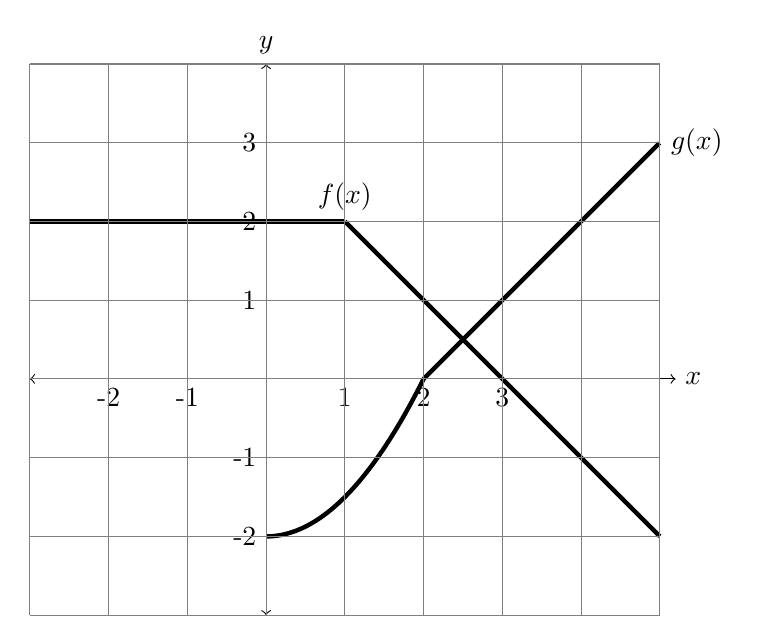
\begin{tikzpicture}[baseline=(current bounding box.center), xscale=1, yscale=1]

\draw[<->] (0,-3) -- (0,4) node[above] {$y$};
\draw[<->](-3,0) -- (5.2, 0) node[right] {$x$};
\foreach \i in {-2,-1, 1, 2,3}{\draw (\i, .1) -- (\i, -.1);
\draw (\i,0) node[below] {\i};
}
\foreach \i in {-2,-1,1,2,3}{
\draw (-.1, \i) -- (.1,\i);
\draw (0,\i) node[  left] {\i};
}
\draw[smooth,samples=200,domain=-3:1, ultra thick]  plot({\x},{2}) node[above]{$f(x)$};
\draw[smooth,samples=200,domain=1:5, ultra thick]  plot({\x},{3-\x});
\draw[smooth,samples=200,domain=0:2, ultra thick]  plot({\x},{(0.5)*(\x)^2-2});
\draw[smooth,samples=200,domain=2:5, ultra thick]  plot({\x},{\x-2}) node[right]{$g(x)$};
\draw[step=1.0,gray,thin] (-3,-3) grid (5,4);
\end{tikzpicture}
\end{center}
\begin{enumerate}
\item $(f+g)(4)$
\vfill
\item $(fg)(0)$
\vfill
\item $(f \circ g)(0)$
\vfill
\item $(g \circ f)(0)$
\vfill
\item $(f \circ g)(4)$
\vfill
\item $(g \circ f)(4)$
\vfill
\item $(f \circ f)(-1)$
\vfill
\item $(f \circ f)(4)$
\vfill
\end{enumerate}
\newpage

{\sc{Example 6}} For each of the following, express the function as a composition of the form $f \circ g$ {\emph{where $g(x) \not=x.$}}
\begin{enumerate}
\item $F(x)=2\sqrt{4+\sqrt{x}}$
\vspace{1in}
\item $H(x)= \frac{1}{x^2+1}$
\vspace{1in}
\item $G(x)=\frac{7x^3}{5+x^3}$
\end{enumerate}

\end{document}

